
\newpage
\section{In-house Algorithmic Profiling}
\label{sec:inhouse}

In this section, we discuss the design and implementation for the in-house version of \Tool.
Under the in-house setting, 
\Tool can help developers conduct algorithmic profiling to detect 
previously unknown complexity problems before releasing their software, 
or help developers diagnose and fix complexity problems reported by end users. 

To conduct algorithmic profiling,
we first need to record \textit{input} size and \textit{cost} for different code constructs 
in multiple program runs;
we then plot records from the same code construct with input size as x-axis and cost as y-axis; 
and finally, we infer a cost function of input size.
To design the in-house version of \Tool, 
we need to answer three fundamental questions:
1) how to design input metrics; 
2) how to design cost metrics;
and 3) how to infer and compare cost functions. 

\subsection{Input Metric Design}
\label{sec:input}

The goal of input metric design is to figure out metrics
holding input size information for different types of code constructs. 
We cannot rely on developers to manually label or specify input size information, 
because it is time-consuming and also difficult for complex code constructs.  
There are several metrics, which can be used to measure input size.
We discuss them as follows. 

\noindent\textbf{Program Input}
As discussed in Section~\ref{sec:process}, 
users tend to specify how to change the whole program 
input to describe the perceived complexity problem.
It is fairly easy to measure input size for the whole program based on users' reports.
One way to measure input size for a code construct
is to simply use the input size of the whole program. 
However, the whole program input 
is related to the input of a code construct in various ways.
Changing the whole program input may not change input sizes for 
all code constructs. 
Using the input size of the whole program as input size for a code 
construct may lead to incorrect profiling results. 

\noindent\textbf{Read Memory Size (RMS)}}
RMS is proposed as an input metric for a dynamic instance
of a code construct~\cite{Aprof1,Aprof2}. 
RMS is defined as the number of distinct memory cells 
whose first access is read. 
RMS considers both reads conducted by a code construct directly 
and reads conducted by 
functions called from the code construct. 
RMS can provide important input information for many complexity problems.   
 
Given a code construct \texttt{c} of a program, 
we assume \texttt{c} is inside a loop \texttt{l} and is executed
$n$ times in one run of the program. 
We would have $n$ RMS records collected for \texttt{c}. 
There are two methods to analyze these $n$ RMS records.
The first method aggregates the $n$ records in a \textit{top-down} way~\cite{Aprof1,Aprof2}.
When analyzing complexity for \texttt{c}, 
we consider the $n$ records independently from each other. 
The effect of multiple executions of \texttt{c} 
will be aggregated when analyzing complexity for \texttt{l}.
The second method aggregates the $n$ records in a \textit{bottom-up} way.
When analyzing complexity for \texttt{c}, 
we merge the $n$ records and calculate the number of distinct memory cells 
contributing RMS as the input size of \texttt{c} during the whole program run.


\begin{figure*}
\centering
\subfloat[XXXX]{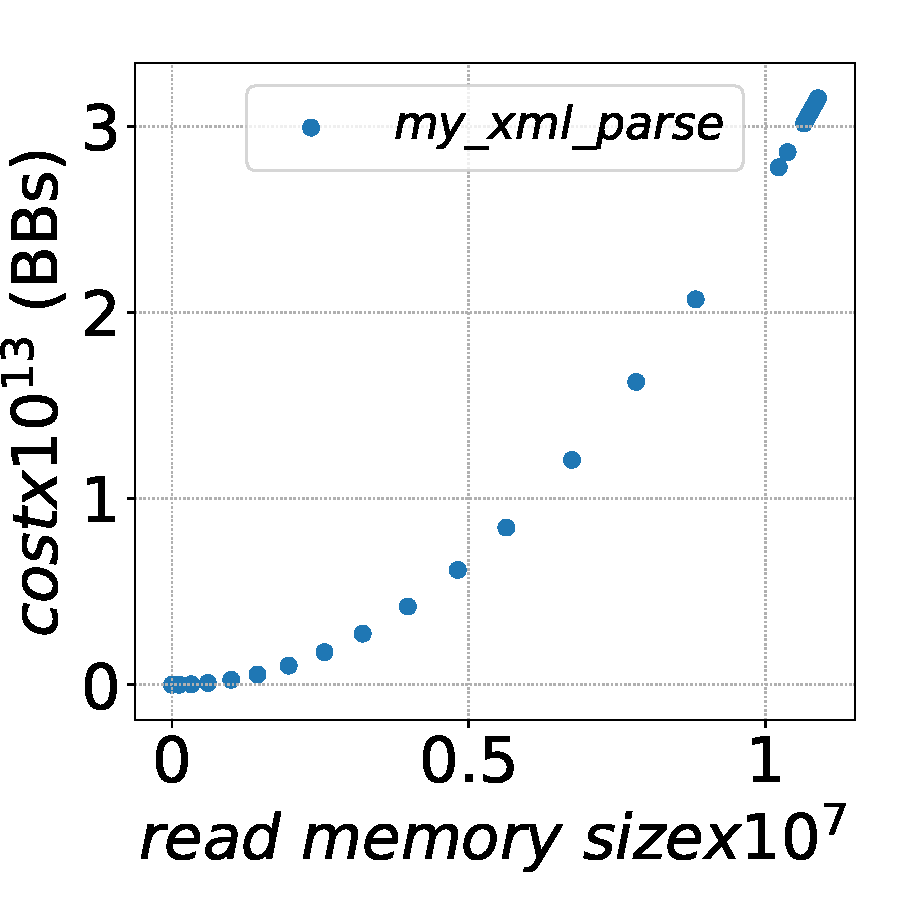
\includegraphics[width=0.22\linewidth]{figure/mysql27287-complexity-n-square}\label{fig:mysql27287-indep}} 
\subfloat[XXXX]{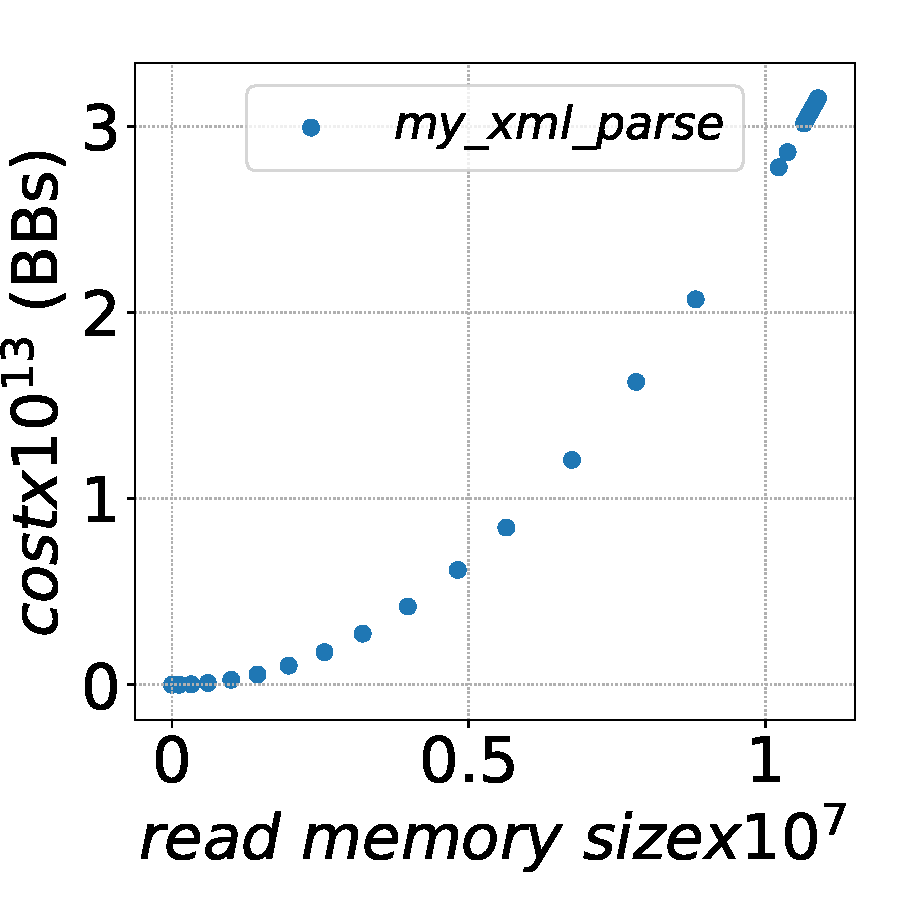
\includegraphics[width=0.22\linewidth]{figure/mysql27287-complexity-n-square}\label{fig:mysql27287-outer}}
\subfloat[XXXX]{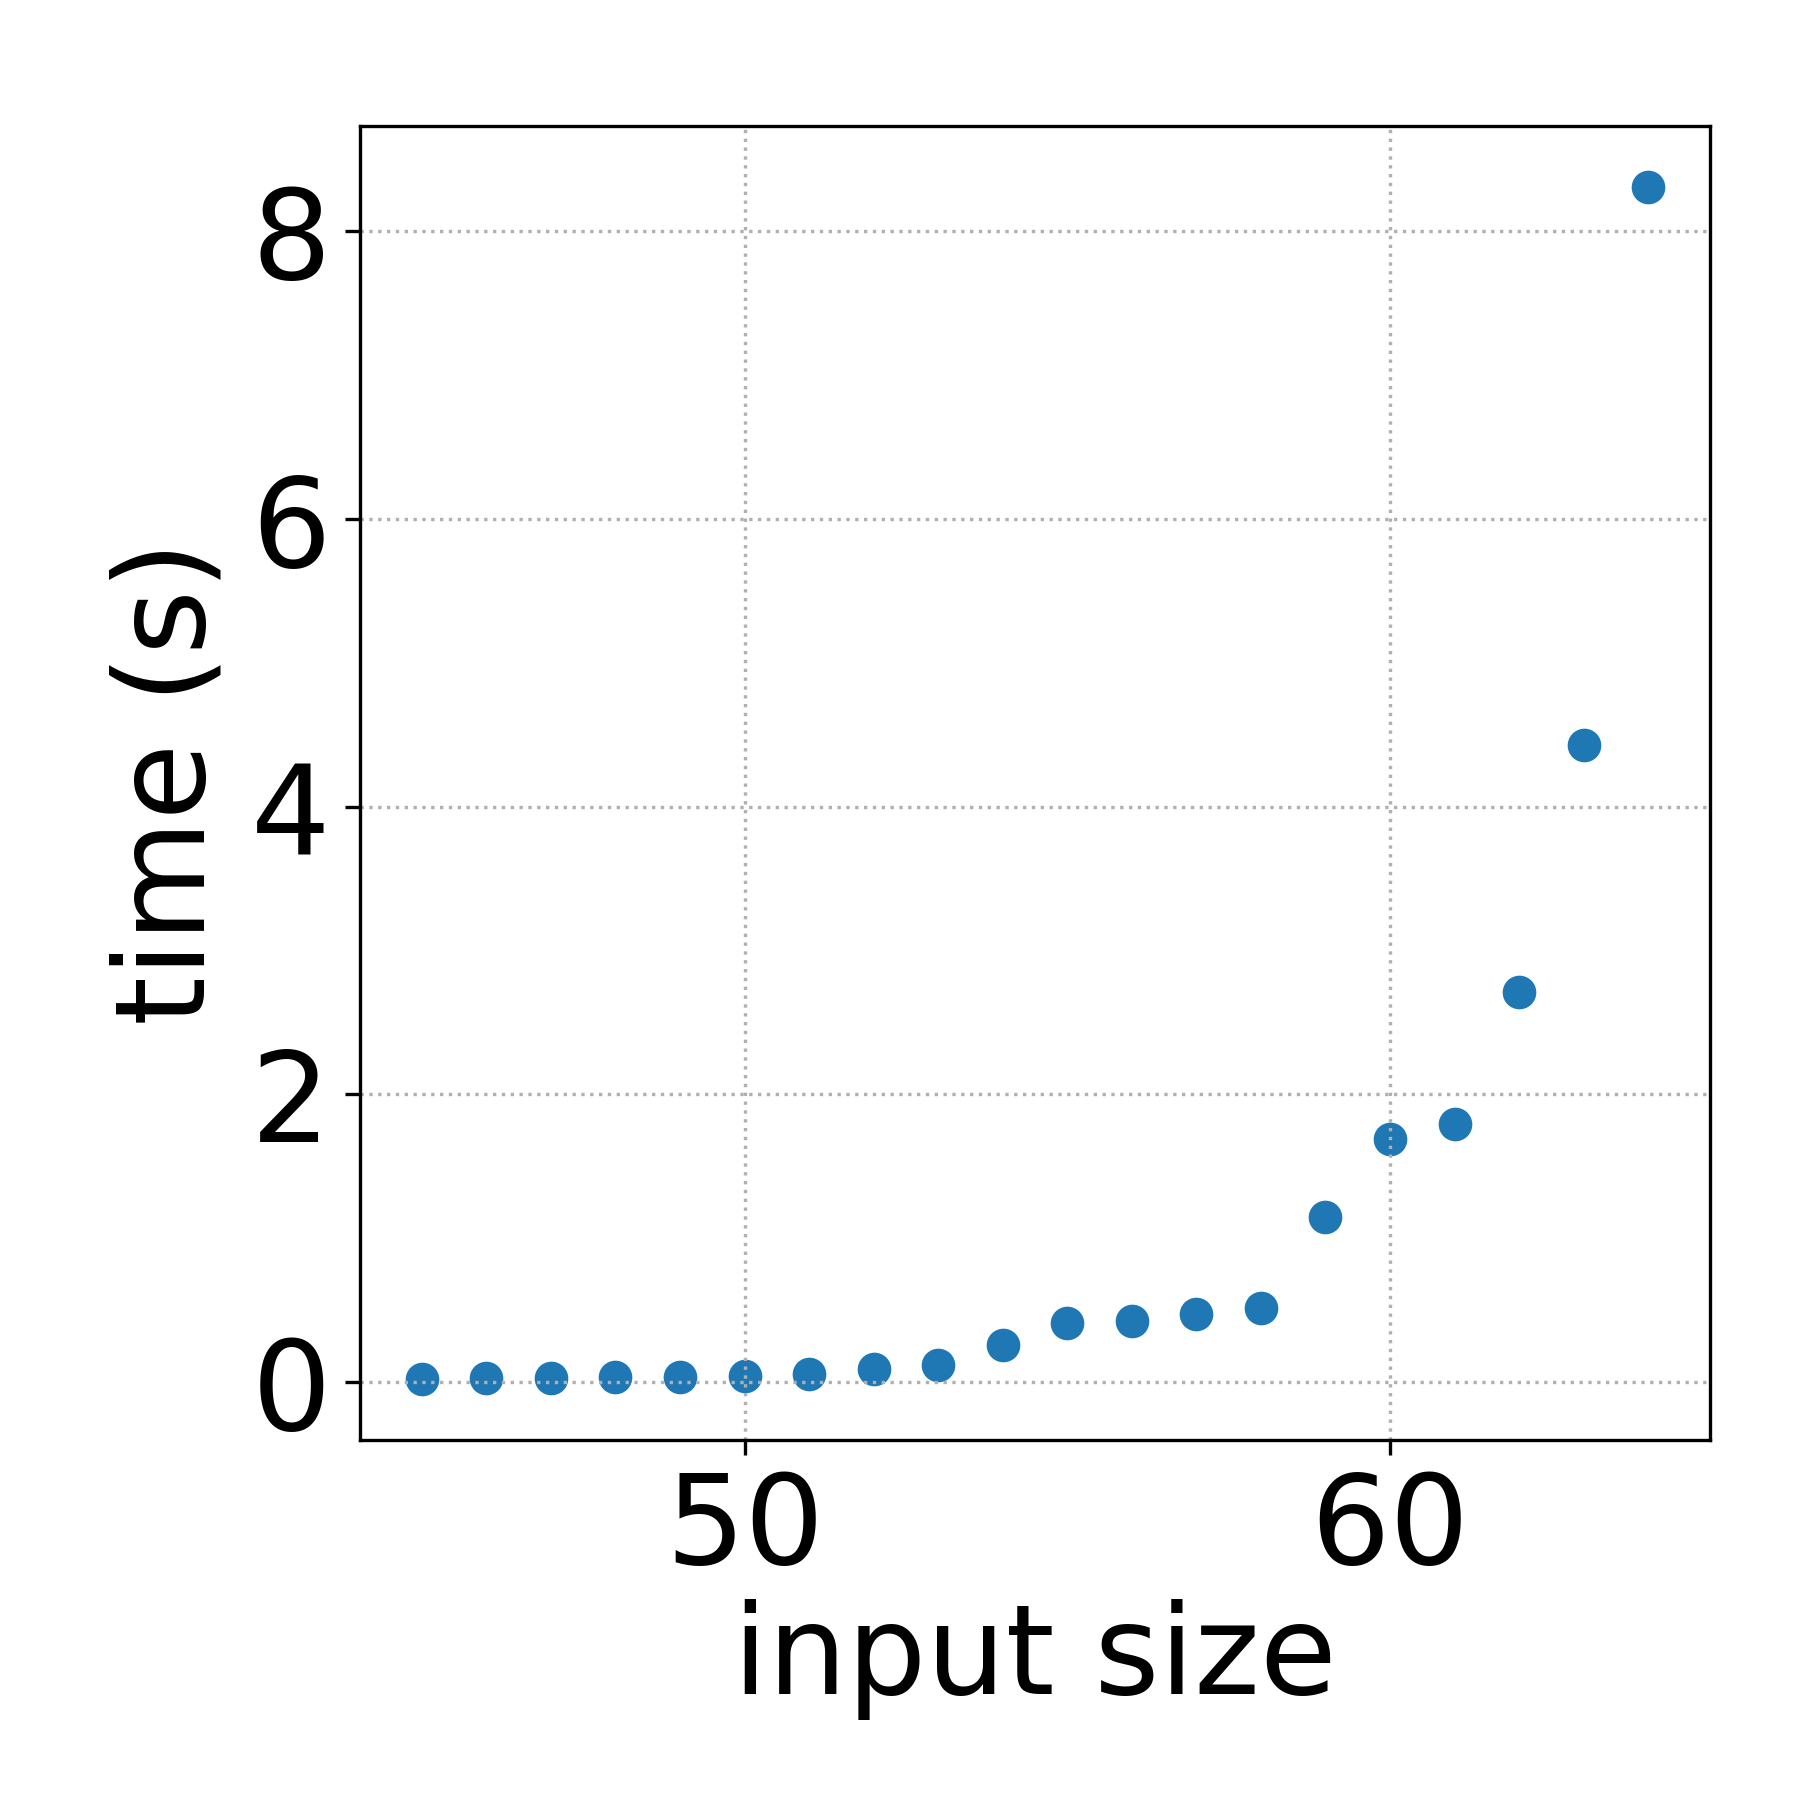
\includegraphics[width=0.22\linewidth]{figure/gcc27733-time-cost-line}\label{fig:mysql27287-merge}} 
\subfloat[XXXX]{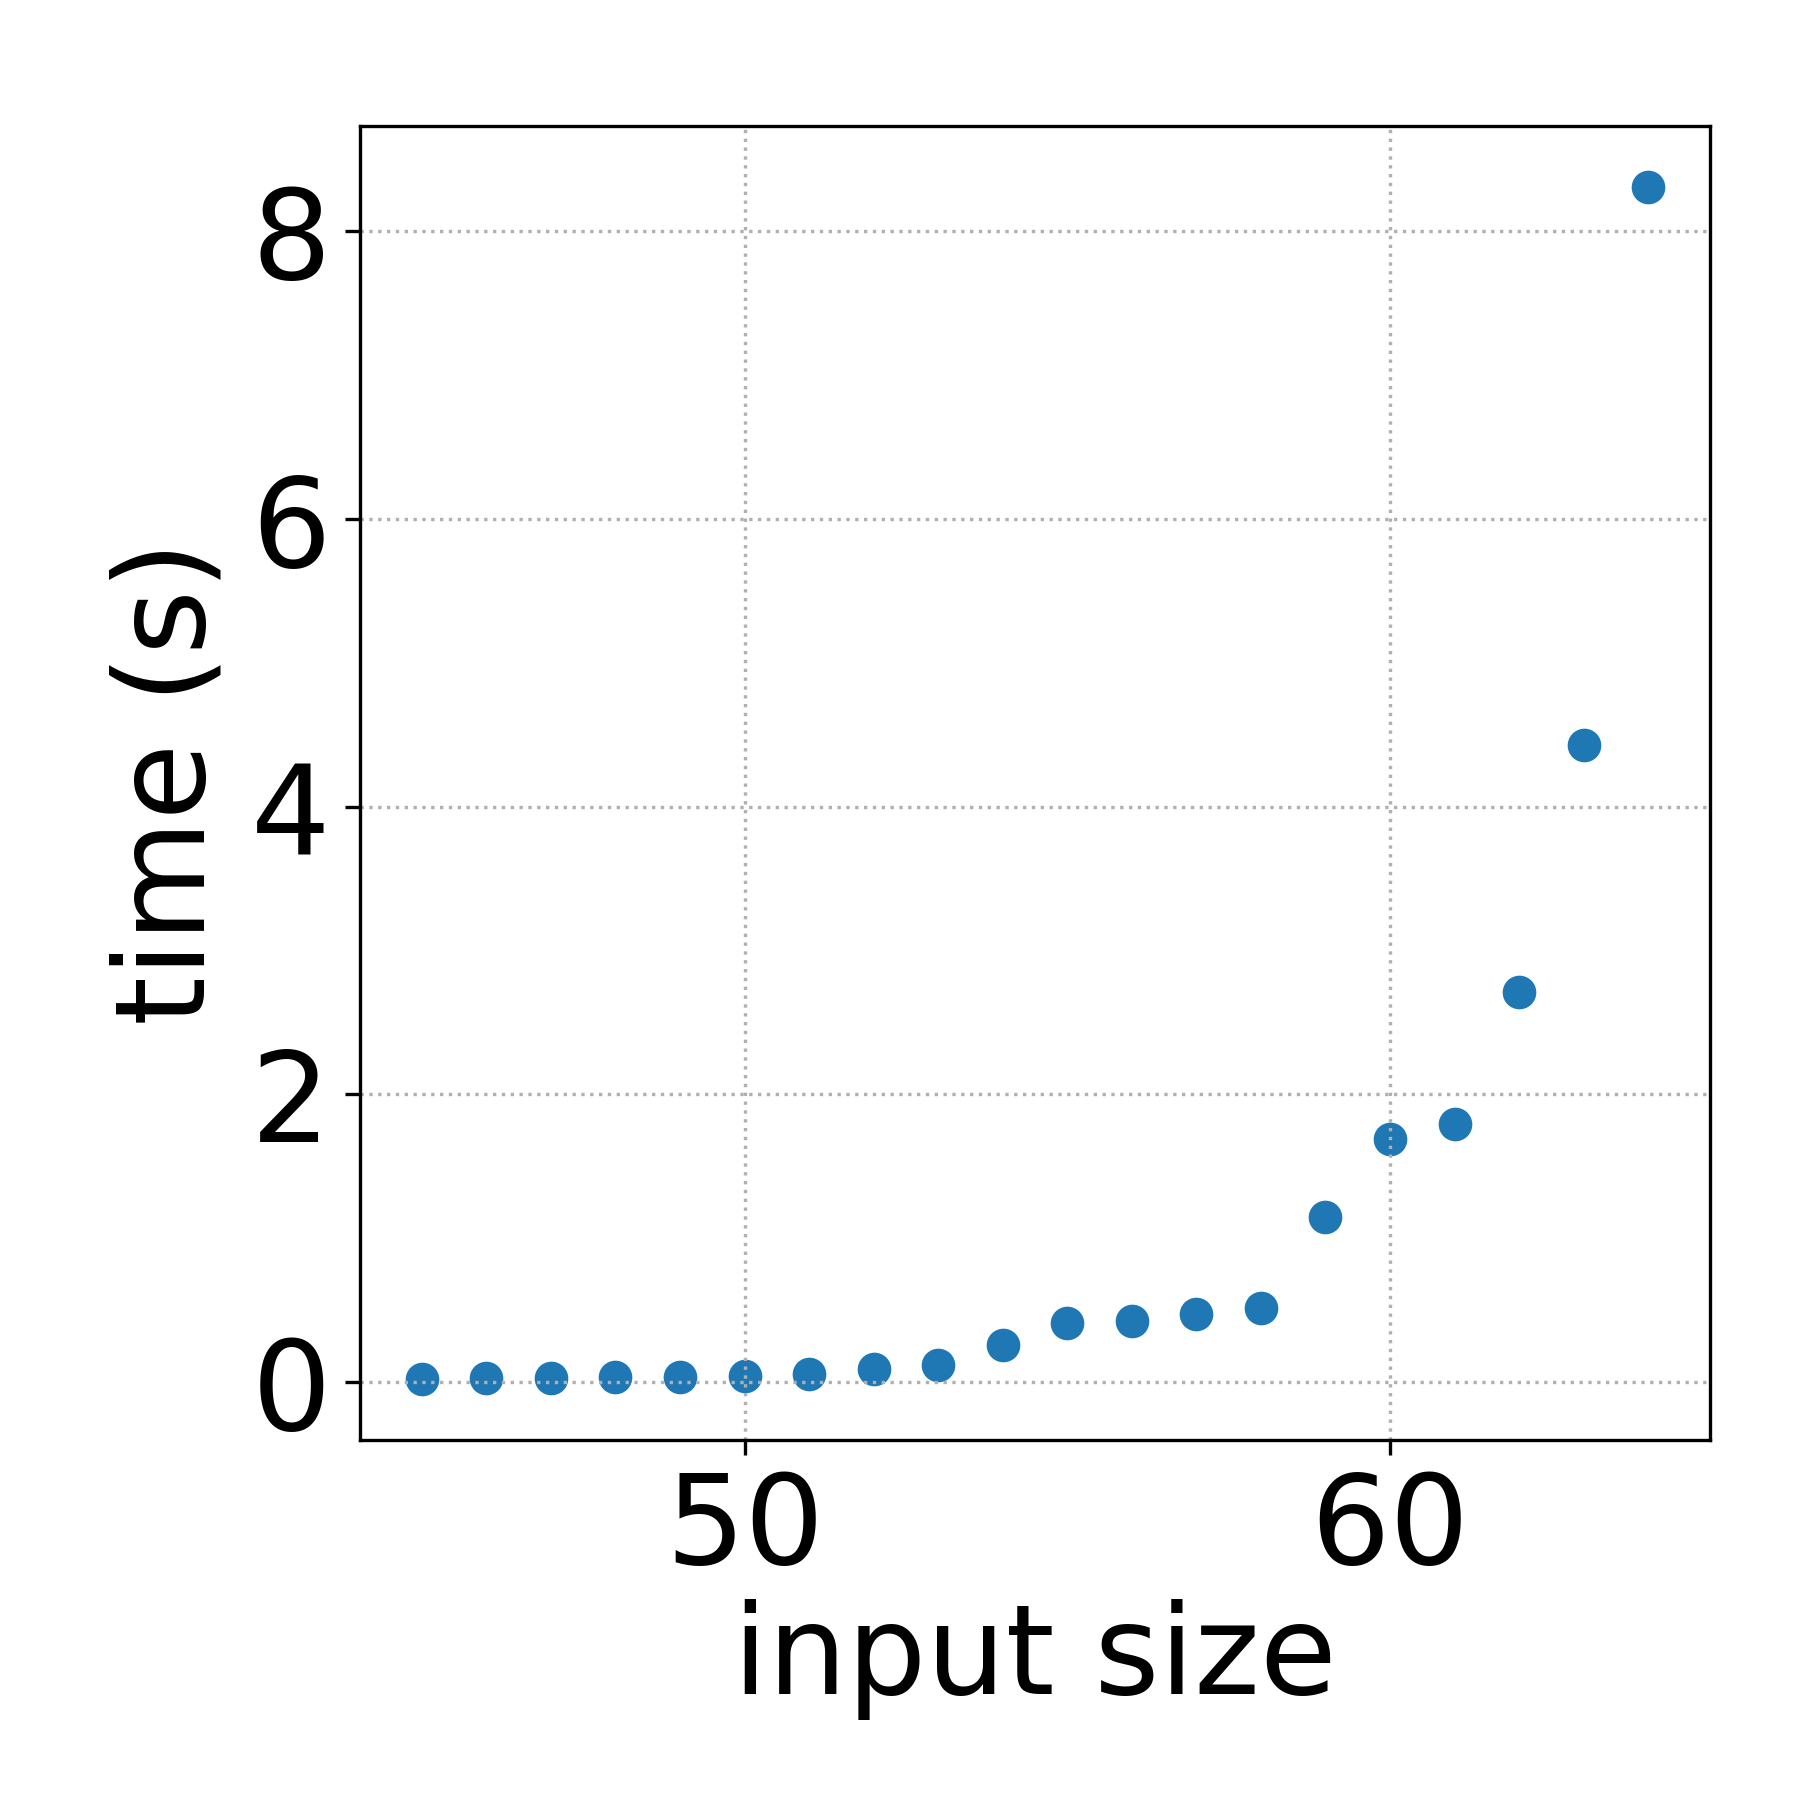
\includegraphics[width=0.22\linewidth]{figure/gcc27733-time-cost-line}\label{fig:mysql27287-inner-array}} \\ 
\vspace{-0.1in}
\caption{XXXX
\footnotesize{(These figures show how execution time change with the change of input size for MySQL\#27287, 
 Apache\#34464, Mozilla\#477564, and GCC\#27733. For each complexity problem, we use 10 distinct inputs.)}} 
\label{fig:time} 
\end{figure*} 

Take MySQL\#27287 as an example.
RMS for one single execution of
the buggy loop in Figure~\ref{fig:mysql27287}
is roughly equal to 2 times the number of \texttt{XML\_NODE}s 
accessed during the execution, 
because the \texttt{level} field and the \texttt{type} field of 
different \texttt{XML\_NODE}s are read in different loop iterations.
Although variable \texttt{p} and \texttt{level} are also read in each iteration,
RMS only considers distinct memory cells and 
only increments its value for the first read on these two variables in the first iteration. 
The outer loop, not shown in Figure~\ref{fig:mysql27287}, 
invokes \texttt{xml\_parent\_tag()} for every \texttt{XML\_NODE} contained
in the same array \texttt{items}.
If we use the top-down method to analyze the buggy loop
or the buggy function, 
execution cost is in linear relationship with RMS, 
as shown in Figure~\ref{fig:mysql27287-indep}.
The $O(N^2)$ complexity can be inferred from the side of the outer loop, 
as shown in Figure~\ref{fig:mysql27287-outer}. 
If we use the bottom-up method, 
we can observe the aggregated cost scales 
polynomially in terms of RMS for the buggy loop 
or the buggy function, 
which is shown in Figure~\ref{fig:mysql27287-merge}. 

\noindent\textbf{Data structure size (DSS)}
The number of distinct accessed elements of a data 
structure could also be used to measure 
input size for a dynamic instance of a code construct~\cite{AlgoProf}. 
As we discussed in Section~\ref{sec:study_impli},
array and linked list are the two types of data structures
most commonly involved in complexity problems. 

Similar to RMS, there are also, top-down and bottom-up, 
two methods to analyze 
multiple DSS records collected for the same code 
construct in one program run.
Take MySQL\#27287 in Figure~\ref{fig:mysql27287} as an example.
If we focus on array \texttt{items},
DSS for one execution of the inner loop is the number of 
accessed array elements during the execution.
If we use the top-down method, the execution cost 
of the inner loop is in linear relationship with its DSS.
For the outer loop, its execution cost is in $O(N^2)$ relationship with its DSS,
since DSS only considers distinct accessed elements.
If we apply the bottom-up method, 
we count distinct accessed array elements across all dynamic instances of the inner loop,
the aggregate execution cost of the inner loop is in $O(N^2)$ relationship with its DSS, 
as shown in Figure~\ref{fig:mysql27287-inner-array}.   

\noindent\textbf{Library input size (LIS)}
There are code constructs taking inputs from library calls. 
As we discussed in Section~\ref{sec:tax}, 
the loop shown in Figure~\ref{fig:apache34464} 
is in $O(N^2)$ complexity in terms of the number 
of characters returned from \texttt{getchar()}. 
Besides \texttt{getchar()}, there are many other library calls, 
which allow code constructs to take inputs
from disk, terminal, network, and many other places. 

LIS can complement RMS for cases like Apache\#34464 in Figure~\ref{fig:apache34464}.
RMS only considers memory cells whose first access is read. 
The first accesses for all memory cells of string \texttt{source} are write on line $8$.
Therefore, all accesses on string 
\texttt{source} will not increase RMS value.  
%If we use RMS to measure input size for the loop in Figure~\ref{fig:apache34464},
RMS for the loop in Figure~\ref{fig:apache34464} only depends 
on the size of string \texttt{target}, 
variable \texttt{sourceLen}, and variable \texttt{targetLen}, 
regardless of the number of characters from \texttt{getchar()}.
DSS can correctly measure input size for Apache\#34464,
since all characters from \texttt{getchar()} will be saved in string (or array) \texttt{source},
and each element of string \texttt{source} 
will be accessed by the inner loop inside \texttt{indexOf()}. 


\begin{figure}
\centering
\lstset{basicstyle=\ttfamily\fontsize{7}{8}\selectfont,
     morekeywords={+},keepspaces=true,numbers=left}
  \mbox{\lstinputlisting[mathescape,boxpos=t]{figure/fib.c}}
\caption{A recursive function exponential complexity.
\footnotesize{(This figure shows a recursive implement to compute fibonacci numbers. 
Execution time scales polynomially in the value of input parameter $n$.)}}
\vspace{-0.05in}
\label{fig:fib}\vspace{-0.05in}
\end{figure}


\noindent\textbf{Important integer variable (IIV)}
Sometimes, a code construct contains some important integer variables,
whose values determine how many times a loop iterates 
or how many times a recursive function is invoked. 
Values of these important integer variables contain important information about input sizes. 
For example, a recursive implementation to calculate fibonacci numbers is shown in Figure~\ref{fig:fib}, 
and it scales exponentially in the value of variable $n$.

IIV can complement RMS, DSS and LIS for cases like 
computing fibonacci numbers in Figure~\ref{fig:fib}. 
If we use RMS to measure input size,
no matter how large \texttt{n} is, the input size will always be constant. 
For an invocation of \texttt{fib},
the first \texttt{read} on parameter \texttt{n} will increase RMS.
After that, RMS will not increase any more.
This is because whenever \texttt{fib} recursively call itself on line 3,
it must write parameter $n-1$ (or $n-2$) onto the stack, 
which means the first access for the stack cell is \texttt{write} 
and future accesses on the stack cell will not increase RMS. 
The recursive function does not
involve any data structure or library call, 
so that it cannot be measure by DSS and LIS. 
 

\paragraph{\textit{\underline{Input metric selection for \Tool}}}
We choose input metrics to explore two directions. 
The first one is to cover as many cases as possible. 
RMS is the most general metric.
RMS can largely cover cases DSS can handle.
We use LIS and IIV to enhance RMS.
We name the enhanced version as RMS+.
The second direction is to find a simple and semantic metric, 
which can cover  a good percentage of common cases. 
We will apply DSS along this direction. 
In the remainder of this paper, 
we will focus on RMS+ and DSS as input metrics. 

\subsection{Cost Metric Design}
When a code construct is executed, 
it could consume many different types of resources, 
such as computation, network bandwidth, storage, and so on.
In this paper, we focus on how to measure computation cost and 
leave the measurement for other types of consumed resources for future works. 
When a code construct is executed, 
there are many metrics can be used to measure computation 
cost for a dynamic instance of the code construct. 
We discuss commonly used ones as follows.

\noindent\textbf{Execution Time}
We can use time elapsed during executing a dynamic instance to present computation cost 
for the instance.
One potential problem to use execution time is that, 
when a dynamic instance takes very little time, 
execution time may fail to provide an accurate measurement.  

\noindent\textbf{Executed Basic Blocks (BBs)}
We can count the number of executed BBs for a dynamic instance
and use this number as computation cost. 
The assumption to use this metric is that 
each executed BB will roughly consume the same computation cost. 

\noindent\textbf{Executed Instructions}
We can use the executed instruction number of a dynamic 
instance to represent computation cost for the instance. 
Similar to executed BBs, we assume each instruction 
roughly takes the same computation cost by using this metric. 


\noindent\textbf{{Loop Iterations (LIs)}}
As we discussed in Section~\ref{sec:study},
many complexity problems are caused by a loop.
If we want to measure computation cost for a loop instance,
we can use the number of loop iterations.
By using this metric, we assume that computation 
cost spent in each iteration is roughly the same. 

\noindent\textbf{Recursive Invocations (RIs)}
As we discussed in Section~\ref{sec:study},
there are also complexity problems caused by recursive functions.
If we want to measure computation cost for a dynamic instance \texttt{d}
of a recursive function \texttt{f}, 
we can use the number of times when
\texttt{d} recursively call \texttt{f} directly or indirectly. 
By using this metric, 
we assume that except the recursive part, 
computation spent in other parts is roughly 
the same across different recursive instances. 

\paragraph{\textit{\underline{Cost metric selection for \Tool}}}
Similar input metrics,
we want both generic cost metrics and cost metrics to cover common cases. 
We use BBs as the generic metric.
We do not use execution time, 
because it is not accurate enough for dynamic instances taking too little time.
We do not use the number of executed instructions, 
because this number is highly correlated with BBs.  
All our studied complexity problems are caused either by a loop or a recursive function. 
Therefore, we will use LIs and RIs as cost metrics for loops and recursive functions, 
respectively.

\subsection{Cost Function Inference and Comparison}

\noindent\textbf{Inference}
After collecting a set of (input size, cost) pairs for a code construct,
we first use maximum cost to aggregate pairs with the same input size into one.
We do this, because we want to infer worst-case complexity for the code construct. 
To infer a cost function,
we consider four possibilities: 
an exponential function, or a polynomial function with degree from 1 to 3.
 We use least square~\cite{least} to determine parameters for the four possible functions. 
For example, we start a polynomial function with degree 2 as $y=a*x^2 + b*x +c$.
We choose $a$, $b$ and $c$ to minimize the sum of squared difference between 
observed value and fitted value.  
To choose the best one among the four possible fitted functions, 
we calculate coefficient of determination for each. 
Coefficient of determination is commonly used to measure goodness-of-fit~\cite{codeter}.
We choose the fitted function with highest coefficient of determination. 


\noindent\textbf{Comparison}
We have more than one metric for both input and cost.
We need to compare functions inferred under different metrics. 
After collecting two sets of records, $a$ and $b$, using different metrics, 
we do the comparison through the following steps. 
We first standardize the two sets of data. 
We then infer two cost functions, $f_a()$ and $f_b()$, 
by using the two sets of standardized data.
We random sample a set of $n$ numbers from $(-1, 1)$.
We use $N$ to represent the set of $n$ sampled numbers.  
We calculate the similarity between the two inferred 
functions by using the following formula. 


%\begin{equation} \label{eq:fun_similarity}
%$1-|f_a(x) - f_b(x)|/(max(f_a(x),f_b(x))+1)$
%\end{equation}

\begin{equation} \label{eq:sim}
%$$p_v(S_v(a)) = 1 - \prod\limits_{u \in S_v(a)}(1 - p_{u,v})$$
S(f_a, f_b) = 1 - \frac{1}{n}\sum_{x \in N}\frac{|f_a(x) - f_b(x)|}{max(f_a(x),f_b(x))+1}
\end{equation}

The intuition of Equation~\ref{eq:sim} is to calculate the area under the two curves 
plotted by $f_a()$ and $f_b()$, 
and compute the similarity as the percentage of the area under both of the two curves, 
compared with the area under either of the two curves.
Since the minimum value of standardized data is $-1$ not $0$,
we minus $-1$ in the denominator.
The maximum value of $S(f_a, f_b)$ is $1$, and the minimum value is $0$.
Larger result means the two functions inferred from $a$ and $b$ are more similar to each other. 



\subsection{Implementation and Optimization}

We use LLVM\cite{llvm} to instrument programs to be profiled.
We use python to analyze profiling records 
with input and cost information and to infer cost function. 
We also design several optimizations to lower runtime overhead 
during dynamic monitoring.  


\subsubsection{Input Metric}
As we discussed in Section~\ref{sec:input},
both RMS+ and DSS have, top-down and bottom-up, 
two methods to analyze profiling records for multiple instances of 
a code construct in one program run. 
Both of these two methods can infer the same complexity, 
such as for MySQL\#27287,
but they require different implementations.
If we want to apply the bottom-up method,
we need to track distinct memory cells already contributing 
RMS+ or DSS for every code construct under monitoring.
During in-house testing, developers usually want to conduct algorithmic profiling 
for all executed code constructs. 
Tracking memory cells for every code construct will 
incur a very large memory overhead.  
As we will discuss later, the top-down method 
is not suitable in production-run usage. 
Therefore, we apply the top-down method under in-house setting, 
and we will use the bottom-up method under production-run setting. 

Since we take the top-down method for in-house setting,
when a monitored program conducts a memory access,
we need to check all functions active on the call stack and 
update information necessary to calculate RMS+ or DSS. 
For simplicity, we use function as granularity for code constructs under in-house setting.
Otherwise, we need to check whether a monitored code construct enclose related call sites, 
when checking active functions on the call stack.  

\paragraph{\textit{\underline{How to implement RMS+}}}
\citet{Aprof1,Aprof2} designed an algorithm to collect 
RMS for all executed functions based on 
Valgrind. We briefly discuss this algorithm firstly, 
and then we will discuss how to enhance this algorithm. 
To count RMS for every function call instance, 
several global variables are maintained: 
\texttt{count}, serving as the current timestamp and incremented 
by 1 after each function invocation,  
\texttt{ts}, a hash table containing the latest access timestamp for each memory cell, 
and \texttt{S}, a shadow stack tracking all active functions on the stack. 
Four hook functions are instrumented for four types of instructions:
\texttt{call}, \texttt{return}, \texttt{read}, and \texttt{write}.
The \texttt{call} hook function will increment the timestamp variable \texttt{count} 
and grow the shadow stack \texttt{S}.
The \texttt{return} hook function will generate a 
log containing information about the returning function's RMS.
The \texttt{read} hook function will query the hash table \texttt{ts} to decide whether 
to increment RMS for all the functions active on the shadow stack \texttt{S}.
Both the \texttt{read} and \texttt{write} hook 
functions will update the hash table \texttt{ts}
by using the value of \texttt{count} to guarantee that \texttt{ts} 
contains the latest access timestamp for each memory cell. 

To enhance RMS with LIS, we keep a list of library functions, which can take inputs.
When these library functions are called,
we will increase RMS by using the size of inputs from these libraries calls 
for all functions active on the call stack. 
To enhance RMS with IIV, 
we consider cases where a function recursively invoke itself using integer parameters. 
We do not instrument \texttt{write} instructions that store integer 
parameters on stack when a function recursively calls itself. 
If the first accesses on these stack memory cells are \texttt{read} 
instructions inside recursive callees, 
they can increase RMS. 
By doing this, we basically use the number of integer parameters 
active simultaneously on the recursive call chain, 
not concrete integer values, as input size.

\paragraph{\textit{\underline{How to implement DSS}}}
To implement DSS, we focus on array and linked list, 
because they are the most common types of data structures in complexity problems. 
We reuse the framework for RMS+ to collect DSS information.
The difference is that we do not instrument \texttt{write} instructions,
and we only instrument \texttt{read} instructions accessing elements 
in an array or a linked list.
We figure out which pointers pointing to elements in an array 
or a linked list through analyzing loops.

Given a pointer, 
if it is deferenced in every iteration of a loop, 
and its value is increased or decreased by an integer value in every iteration,
we consider the pointer points to array elements, 
and the loop is an array-processing loop. 
For example, as shown in Figure~\ref{fig:mysql27287}, 
\texttt{p} points to array elements. 
It is deferenced in every iteration of the loop in Figure~\ref{fig:mysql27287},
and its value is decreased by one in every iteration. 

For a pointer pointing to elements in a linked list,
its base type needs to be a \texttt{struct}. 
The pointer is also deferenced in every iteration of a loop.
Its value is updated in every iteration, 
and its new value is one field of the \texttt{struct} it is pointing to. 
After identifying a pointer pointing to linked list elements,
we consider the loop deferencing the pointer and updating its value as 
a linked-list-processing loop. 
For example, \texttt{n} is deferenced in every iteration of the loop
in Figure~\ref{fig:Mozilla477564}. 
Its value is also updated in every iteration by 
using the \texttt{prev} field of \texttt{node\_t} it is pointing to. 
We will identify \texttt{n} pointing to elements in a linked list,
and the loop shown in Figure~\ref{fig:Mozilla477564} as a linked-list-processing loop.

\paragraph{\textit{\underline{How to do optimization}}}
We design three optimizations to reduce the runtime overhead when collecting input information
from two aspects:
we try to reduce the number of instrumentation sites, 
and we try to accelerate hook functions. 


\noindent\textbf{Optimization 1}
The first optimization is designed for RMS+,
and it targets to reduce the number of instrumentation sites 
for \texttt{read} and \texttt{write} instructions. 
The \texttt{read} hook function needs to query hash table \texttt{ts} 
to get the timestamp for the latest access and update RMS+ value when necessary. 
Both \texttt{read} and \texttt{write} hook functions 
need to use the value of \texttt{count} to update hash table \texttt{ts}.
As we discussed earlier, the value of texttt{count} will be increased 
after each function invocation. 
Therefore, given two consecutive memory accesses on the same memory cell,
if there is no function calls between them, 
we do not need to instrument the second memory access. 

We rely on dominance analysis to implement this optimization. 
We focus on stack memory cells that hold 
scalar variables and only have \texttt{read} and \texttt{write} as uses 
(i.e., not having ``address of'' as uses).
We only focus on these memory cells,
because we want to avoid pointer alias analysis, 
which may potentially introduce inaccurate results. 
For a \texttt{read} or \texttt{write} instruction on one of these memory cells,
if it is dominated by another \texttt{read} or \texttt{write} instruction on the same cell, 
and there is not function call on any path between these two instructions,
we will skip the instrumentation for the second instruction.  

\noindent\textbf{Optimization 2}}
The second optimization is an attempt to improve the performance of 
lookups in the hash table \texttt{ts}, 
containing the latest access timestamp for each memory cell.
It can work for both RMS+ and DSS.
For a memory read, 
we need to query \texttt{ts} and decide 
whether RMS+ or DSS should be incremented.
For both memory read and write, 
we need to update \texttt{ts} by using the current timestamp \texttt{count}
for accessed memory cells. 

Instead of using a hash table, 
we use a page table to contain the timestamp information. 
To balance runtime overhead and memory overhead, 
we design a four-layer page table for 32-bit programs.
We use 4-KB consecutive memory areas to hold pointers pointing to 
memory areas in the next layer 
or memory areas holding timestamps for memory cells. 
For a monitored 32-bit program, 
we need to calculate four addresses using bitwise operations 
and use the four addresses to refer to each layer of the page table.  
For 64-bit programs, we use six layers.  
Compared with the hash table, 
the page table leverages the locality of memory accesses 
and can lead 
to a better cache performance. 
To further improve performance, 
we add an extra variable to hold the pointer pointing 
to the last referenced memory area holding timestamps.
For each memory read or write, 
we first check whether the saved pointer value can be used. 
We only conduct a page table lookup when the saved value cannot be used. 

\noindent\textbf{Optimization 3}
For this optimization, we apply inline functionality 
provided by LLVM to make all instrumented hook functions inline.

\subsubsection{Cost Metric}
To count LIs, for every monitored loop, we initialize 
a global counter to be 0 at the beginning of the program and 
increase the counter by $1$ in the loop header to count the number of iterations.
To count RIs, for each monitored recursive function, 
we initialize a global counter to be 0 at the beginning of the program
and increase the counter 
in the entry block of the recursive function 
to count the number of recursive instances. 
To count BBs, a naive method is to create a global counter
and increase the counter value in every basic block. 



\noindent\textbf{Optimization 4}
To efficiently count executed BBs, 
we apply an algorithm, which was originally designed to 
efficiently count edge events through selectively instrumenting a counter 
on CFG~\cite{event-counting}.
The algorithm has already been proved to be able to 
conduct path profiling efficiently~\cite{peter-ase,path-profiling}. 

To apply the algorithm,
we instrument a local counter \texttt{local\_cost} for each function
and initialize its value to be 0 at the entry BB. 
We will add the value of \texttt{local\_cost} to a global counter \texttt{cost} 
at the exit BB.
After that, we only need to consider where 
and how to update \texttt{local\_cost} 
within a single function.
We design and implement an intra-procedural control flow analysis
to achieve this.
Given a single function,
we add a fake edge from the exit BB to the entry BB 
to make its CFG strongly connected. 
Since the original algorithm is design to count edge events,
we split each BB into two 
and label the event number to be 1 for each edge connecting a pair of split BBs 
We label the event number to be 0 for all other edges.
We compute a spanning tree~\cite{spanning} for the new CFG.
Edges not in the spanning tree are called chords.
We apply the depth-first search algorithm proposed in~\cite{event-counting} 
to calculate on which chords we should change 
\texttt{local\_cost} 
and how much we should change.

\subsection{Experimental Evaluation}
\label{sec:inhouse_exp}
%\subsubsection{Methodology}

\noindent\textbf{Implementation and Platform}
We implement \Tool by using LLVM-5.0.0.
Our current implementation focus on C/C++ programs, 
but we believe that our algorithms are general enough to be extended 
to other programming languages.
We conduct our experiments using a Ubuntu-16.04 machine, 
with i7-7700 CPU and 32-GB memory. 

%\begin{table}[h!]
  \centering
  \scriptsize
  \newcommand{\Yes}[1]{\checkmark{}$_#1$}
  \newcommand{\No}[0]{-}
  \begin{tabular}{lccccccccccc}
    \toprule     
    {\bf BugID}                   & KLOC  &  P.L.    & \multicolumn{6}{c}{\# of Static Features}                      &   Complexity  & Buggy C.C.        & \# of Inputs \\
                           
    \cmidrule(lr){4-9}
                                  &       &          &  BB      &  Loop     & A-L    &  LL-L    &  Function  & R.F.          &           &        &  \\
    \midrule 

    Mozilla\#347306              &  $88$    & C        &   46735  &   1177     &  483    &  136    &  1988  & 35   &  $O(N^{2})$                         &  A-L  & 10000   \\
    Mozilla\#416628              &  $105$   & C        &   46097  &   1116     &  484    &  136    &  1919  &  35  &  $O(N^{2})$                         &  LL-L & 380  \\
    Mozilla\#490742              &  $0.157^*$    & JS         &  41     & 4       &  3     &   0  &  8           &  0   & $O(N)$        &  A-L  &  10000              \\
    Mozilla\#35294               &  $0.195^*$  & C++  & 85 &  9  &  5  & 0  & 12   & 0                                  &  $O(N^{2})$   &  Loop & 50000  \\
    Mozilla\#477564              &  $0.116^*$  & JS  & 40 & 6 & 1 & 3 & 5   & 0                                         & $O(N^{2})$    &  LL-L & 4000       \\
    \midrule
    MySQL\#27287                 &  $995$  & C++  & 88971  & 2535 & 905 & 287 & 11969 & 80                                                          & $O(N^{2})$    & A-L   & 65536            \\
    MySQL\#15811      &  $1127$ & C++  & 17656 & 844 & 237 & 29 & 490 & 5                                                                &  $O(N^{2})$   & A-L   & 16384 \\
    \midrule
    Apache\#37184     &  $0.092^*$ & Java  & 31 & 5  & 0 & 0 & 7 & 0                                                    & $O(N)$        & Loop & 10000     \\ 
    Apache\#29743     &  $0.257^*$  & Java  & 408 & 8 & 0 & 0 & 123 & 0                                                 & $O(N^{2})$    & Loop & 10000 \\
    Apache\#34464     &  $0.16^*$  & Java  & 70 & 6 & 5 & 0  & 13 & 0                                                   & $O(N^{2})$    & A-L  & 50000 \\
    Apache\#47223     &  $0.162^*$ & Java  & 67 & 5 & 4 & 0  & 13 & 0                                                   & $O(N^{2})$    & A-L  & 50000 \\
    \midrule
    GCC\#46401        &  $5521$  & C  & 301913 & 11266 & 1340 & 1637 & 27733 & 964                                                       & $O(N^{2})$    & LL-L & 1462 \\
    GCC\#1687         &  $2099$  & C  & 125408 & 5315  & 724 & 1086  & 7573  & 558                                                       & $O(2^{N})$    & R.F. & 16  \\
    GCC\#27733        &  $3217$  & C  & 217239 & 7412 & 1004 & 1196  & 12722 & 686                                                       & $O(2^{N})$    & R.F. & 65  \\
    GCC\#8805         &  $2538$  & C  & 148099 & 5857 & 841 & 1222 & 6753 & 517                                                          & $O(N^{2})$    & LL-L & 1000 \\
    GCC\#21430        &  $3844$  & C  & 283675 & 7727 & 883  & 1178 & 13745 & 700                                                        & $O(N^{2})$    & LL-L & 10000 \\
    GCC\#12322        &  $2341$  & C  & 124310 & 5397 & 831 & 1190 & 7078 & 540                                                          & $O(N^{2})$    & LL-L & 1175 \\
    \midrule
    \midrule
    Apache\#53622     & $1.094^*$  & Java  & 345 & 38 & 22 & 12 & 72 & 0                                                & $O(N^{2})$    & A-L & 50000    \\
    Apache\#53637     & $0.937^*$  & Java  & 308 & 34 & 21 & 9  & 60 & 0                                                & $O(N^{2})$    & A-L & 50000 \\
    Apache\#53803     & $0.421^*$  & Java  & 128 & 11 & 9  & 0  & 34 & 0                                                & $O(N^{2})$    & A-L & 50000     \\
    Apache\#53821     & $0.417^*$  & Java  & 131 & 12 & 10 & 0  & 34 & 0                                                & $O(N^{2})$    & A-L & 50000      \\
    Apache\#53822     & $0.417^*$  & Java  & 132 & 12 & 11 & 0  & 34 & 0                                                & $O(N^{2})$    & A-L & 50000      \\
    \midrule
    Collections\#406      & $0.253^*$  & Java  & 81 & 9 & 7 & 0 & 19 & 0                                                  & $O(N^{2})$ & A-L & 50000      \\
    Collections\#407      & $0.766^*$  & Java  & 234 & 26 & 15 & 9 & 53 & 0                                               & $O(N^{2})$ & A-L & 50000   \\
    Collections\#408      & $0.742^*$  & Java  & 225 & 25 & 14 & 9 & 51 & 0                                               & $O(N^{2})$ & A-L & 50000    \\
    Collections\#409      & $0.781^*$  & Java  & 236 & 26 & 15 & 9 & 53 & 0                                               & $O(N^{2})$ & A-L & 50000     \\
    Collections\#410      & $0.769^*$ & Java   & 234 & 26 & 15 & 9 & 51 & 0                                               & $O(N^{2})$ & A-L & 50000    \\
    Collections\#412      & $0.284^*$  & Java  & 84 & 9  & 6  & 0  & 20 & 0                                               & $O(N^{2})$ & A-L & 50000     \\
    Collections\#413      & $0.923^*$  & Java  & 274 & 32 & 16 & 14 & 62 & 0                                              & $O(N^{2})$ & LL-L & 50000   \\
    Collections\#425      & $0.758^*$  & Java  & 233 & 26 & 15 & 9  & 52 & 0                                              & $O(N^{2})$ & A-L & 50000    \\
    Collections\#426      & $0.783^*$  & Java  & 242 & 26 & 15 & 9  & 53 & 0                                              & $O(N^{2})$ & A-L & 50000   \\
    Collections\#427      & $0.756^*$ & Java  & 227 & 25 & 14 & 9  & 53 & 0                                               & $O(N^{2})$ & A-L & 50000   \\
    Collections\#429-0    & $0.668^*$  & Java  & 203 & 21 & 11 & 7 & 45 & 0                                             & $O(N^{2})$ & Loop & 30000       \\
    Collections\#429-1    & $0.536^*$  & Java  & 157 & 20 & 13 & 4 & 36 & 0                                             & $O(N^{2})$ & Loop & 30000     \\
    Collections\#429-2    & $0.416^*$ & Java  & 129 & 15 & 9 & 3  & 26 & 0                                             & $O(N^{2})$ & Loop & 30000 \\
    Collections\#434      & $0.336^*$  & Java  & 86  & 10 & 0 & 8 & 33 & 0                                               & $O(N^{2})$ & LL-L & 50000     \\
    \midrule
    Groovy\#5739-0        & $0.745^*$  & Java  & 227 & 10 & 0 & 8 & 51 & 0                                                & $O(N^{2})$ & LL-L& 50000 \\
    Groovy\#5739-1        & $0.756^*$  & Java  &227  & 25 &  14 & 9 & 51 & 0                                              & $O(N^{2})$ & A-L & 50000 \\
    \midrule
    \midrule
    knapsack      &  $0.282$  & C++  & 42 & 1 & 0 & 0 & 5 & 1                                                                            & $O(2^{N})$ & R.F. & 30  \\
    fib      &  $0.048$ & C++  & 10 & 0 & 0 & 0 & 3 & 1                                                                                  & $O(2^{N})$ & R.F. & 45 \\
    parentheses      & $0.056$   & C++  & 10 & 0 & 0 & 0 & 3 & 1                                                                         & $O(2^{N})$ & R.F. & 19 \\
    nqueens      & $0.091$  & C++  & 33 & 3 & 2 & 0 & 4 & 1                                                                              & $O(2^{N})$ & R.F. & 13 \\
    graphcol      &  $0.171$  & C++  & 58 & 8 & 3 & 0 & 8 & 1                                                                            & $O(2^{N})$ & R.F. & 50 \\
    uts      &  $0.667$  & C++  & 40  & 2 & 0 & 0 & 8 & 1                                                                                & $O(N)$     & R.F. & 20 \\
    binomial      &  $0.058$  & C++  & 14 & 0 & 0 & 0 & 3 & 1                                                                            & $O(2^{N})$ & R.F. & 36 \\
    minmax      &  $0.262$  & C++  & 203 & 8 & 3 & 0 & 8 & 1                                                                             & $O(2^{N})$ & R.F. & 13 \\


    \bottomrule
   \end{tabular}
  %\nocaptionrule
  \caption{Benchmark Information.
  \footnotesize{(This table shows information for complexity problems used in our evaluation. 
   $x^*$: thousands of lines of codes for re-implemented benchmarks; 
   A-L: array-processing loop; 
   LL-L: linked-list-processing loop; 
   R.F.: recursive function; 
   Buggy C.C.: buggy code construct.)}}
  \label{tab:benchmark_info}
\end{table}

\noindent\textbf{Benchmarks}
%\Tool is an algorithmic profiling tool chain.
%Developers can use \Tool to diagnose user-perceived performance failures caused by complexity problems, 
%in both in-house and production-run settings. 
%Therefore, we use known complexity problems in the real world to evaluate \Tool. 
To thoroughly conduct our evaluation, 
we select complexity problems from three sources, as shown in Table~\ref{tab:benchmark_info}. 

The first source is our studied complexity problems, 
which are randomly sampled from representative applications in previous works~\cite{PerfBug,SongOOPSLA2014}.
We successfully reproduce 17 complexity problems. 
Among them, 6 bugs are extract from original Java or JS programs, 
and re-implemented by using C/C++, 
because our current implementation of \Tool can only work on C/C++ programs.
One reproduced bug is extract from a very old Mozilla version, 
and we fail to find dependent libraries to build that version. 
We do the re-implementation after we thoroughly understand the complexity problems.
During the re-implementation, we keep the original algorithms, 
data structures, and caller-callee relationships. 
We fail to reproduce other complexity problems, 
because they depend on very special software or hardware environments, 
which are not available to us. 
We fail to re-implement them, 
because their data structures are too complex to extract.

The second source is from Toddler project~\cite{Alabama}. 
Toddler is a dynamic technique that can detect inefficient loops in Java programs.
In a previous work, \citet{ldoctor} re-implemented all 
21 bugs detected by Toddler and verified by developers in C/C++.
During the re-implementation, the researchers first reproduced all Java bugs, 
then they referred JDK to re-implement 
common data structures, like ArrayList, HashMap and Vector, 
and finally, they re-implemented the performance bugs according to their root cases. 
We use the 21 re-implemented bugs in our evaluation.  

The third source is from a previous work, 
which optimizes recursive programs by leveraging SIMD instructions~\cite{ren-bin}. 
8 benchmarks are used in their evaluation part. 
All of the benchmarks are recursive implementation for classic algorithms, 
such as computing fibonacci number, knapsack, nqueens, and so on. 
All their benchmarks are in C++. 
We use all of them in our experiments. 

In total, we evaluate \Tool on 46 benchmarks. 
Information for all benchmarks is shown in Table~\ref{tab:benchmark_info}.
In general, benchmarks used in our experiments are large. 
Except 5 benchmarks, all other benchmarks are more than 100 lines of codes. 
7 benchmarks contain more than 1 million lines of codes. 
We implement a set of simple static analyzers to count static features for these benchmarks. 
For large benchmarks, 
they could contain more than 10 thousand loops and functions.
Algorithmic profiling tools are needed by developers to 
analyze different code constructs automatically.
We also count how many array-processing loops, 
linked-list-processing loops, and recursive functions for each benchmark.
These code constructs are most common root causes for 
benchmarks used in our evaluation.  
The majority of benchmarks used in our experiments are in $O(N^2)$ complexity. 
We also 10 benchmarks in $O(2^N)$ complexity, and 2 benchmarks in $O(N)$ complexity. 

\noindent\textbf{Experimental Setting}

\begin{table}[h!]
  \centering
  \scriptsize
  \newcommand{\Yes}[1]{\checkmark{}$_#1$}
  \newcommand{\No}[0]{-}
  \begin{tabular}{lccccccccccc}
    \toprule     
    {\bf BugID}                   & KLOC  &  P.L.    & \multicolumn{6}{c}{\# of Static Features}                      &   Complexity  & Buggy C.C.        & \# of Inputs \\
                           
    \cmidrule(lr){4-9}
                                  &       &          &  BB      &  Loop     & A-L    &  LL-L    &  Function  & R.F.          &           &        &  \\
    \midrule 

    Mozilla\#347306              &  $88$    & C        &   46735  &   1177     &  483    &  136    &  1988  & 35   &  $O(N^{2})$                         &  A-L  & 10000   \\
    Mozilla\#416628              &  $105$   & C        &   46097  &   1116     &  484    &  136    &  1919  &  35  &  $O(N^{2})$                         &  LL-L & 380  \\
    Mozilla\#490742              &  $0.157^*$    & JS         &  41     & 4       &  3     &   0  &  8           &  0   & $O(N)$        &  A-L  &  10000              \\
    Mozilla\#35294               &  $0.195^*$  & C++  & 85 &  9  &  5  & 0  & 12   & 0                                  &  $O(N^{2})$   &  Loop & 50000  \\
    Mozilla\#477564              &  $0.116^*$  & JS  & 40 & 6 & 1 & 3 & 5   & 0                                         & $O(N^{2})$    &  LL-L & 4000       \\
    \midrule
    MySQL\#27287                 &  $995$  & C++  & 88971  & 2535 & 905 & 287 & 11969 & 80                                                          & $O(N^{2})$    & A-L   & 65536            \\
    MySQL\#15811      &  $1127$ & C++  & 17656 & 844 & 237 & 29 & 490 & 5                                                                &  $O(N^{2})$   & A-L   & 16384 \\
    \midrule
    Apache\#37184     &  $0.092^*$ & Java  & 31 & 5  & 0 & 0 & 7 & 0                                                    & $O(N)$        & Loop & 10000     \\ 
    Apache\#29743     &  $0.257^*$  & Java  & 408 & 8 & 0 & 0 & 123 & 0                                                 & $O(N^{2})$    & Loop & 10000 \\
    Apache\#34464     &  $0.16^*$  & Java  & 70 & 6 & 5 & 0  & 13 & 0                                                   & $O(N^{2})$    & A-L  & 50000 \\
    Apache\#47223     &  $0.162^*$ & Java  & 67 & 5 & 4 & 0  & 13 & 0                                                   & $O(N^{2})$    & A-L  & 50000 \\
    \midrule
    GCC\#46401        &  $5521$  & C  & 301913 & 11266 & 1340 & 1637 & 27733 & 964                                                       & $O(N^{2})$    & LL-L & 1462 \\
    GCC\#1687         &  $2099$  & C  & 125408 & 5315  & 724 & 1086  & 7573  & 558                                                       & $O(2^{N})$    & R.F. & 16  \\
    GCC\#27733        &  $3217$  & C  & 217239 & 7412 & 1004 & 1196  & 12722 & 686                                                       & $O(2^{N})$    & R.F. & 65  \\
    GCC\#8805         &  $2538$  & C  & 148099 & 5857 & 841 & 1222 & 6753 & 517                                                          & $O(N^{2})$    & LL-L & 1000 \\
    GCC\#21430        &  $3844$  & C  & 283675 & 7727 & 883  & 1178 & 13745 & 700                                                        & $O(N^{2})$    & LL-L & 10000 \\
    GCC\#12322        &  $2341$  & C  & 124310 & 5397 & 831 & 1190 & 7078 & 540                                                          & $O(N^{2})$    & LL-L & 1175 \\
    \midrule
    \midrule
    Apache\#53622     & $1.094^*$  & Java  & 345 & 38 & 22 & 12 & 72 & 0                                                & $O(N^{2})$    & A-L & 50000    \\
    Apache\#53637     & $0.937^*$  & Java  & 308 & 34 & 21 & 9  & 60 & 0                                                & $O(N^{2})$    & A-L & 50000 \\
    Apache\#53803     & $0.421^*$  & Java  & 128 & 11 & 9  & 0  & 34 & 0                                                & $O(N^{2})$    & A-L & 50000     \\
    Apache\#53821     & $0.417^*$  & Java  & 131 & 12 & 10 & 0  & 34 & 0                                                & $O(N^{2})$    & A-L & 50000      \\
    Apache\#53822     & $0.417^*$  & Java  & 132 & 12 & 11 & 0  & 34 & 0                                                & $O(N^{2})$    & A-L & 50000      \\
    \midrule
    Collections\#406      & $0.253^*$  & Java  & 81 & 9 & 7 & 0 & 19 & 0                                                  & $O(N^{2})$ & A-L & 50000      \\
    Collections\#407      & $0.766^*$  & Java  & 234 & 26 & 15 & 9 & 53 & 0                                               & $O(N^{2})$ & A-L & 50000   \\
    Collections\#408      & $0.742^*$  & Java  & 225 & 25 & 14 & 9 & 51 & 0                                               & $O(N^{2})$ & A-L & 50000    \\
    Collections\#409      & $0.781^*$  & Java  & 236 & 26 & 15 & 9 & 53 & 0                                               & $O(N^{2})$ & A-L & 50000     \\
    Collections\#410      & $0.769^*$ & Java   & 234 & 26 & 15 & 9 & 51 & 0                                               & $O(N^{2})$ & A-L & 50000    \\
    Collections\#412      & $0.284^*$  & Java  & 84 & 9  & 6  & 0  & 20 & 0                                               & $O(N^{2})$ & A-L & 50000     \\
    Collections\#413      & $0.923^*$  & Java  & 274 & 32 & 16 & 14 & 62 & 0                                              & $O(N^{2})$ & LL-L & 50000   \\
    Collections\#425      & $0.758^*$  & Java  & 233 & 26 & 15 & 9  & 52 & 0                                              & $O(N^{2})$ & A-L & 50000    \\
    Collections\#426      & $0.783^*$  & Java  & 242 & 26 & 15 & 9  & 53 & 0                                              & $O(N^{2})$ & A-L & 50000   \\
    Collections\#427      & $0.756^*$ & Java  & 227 & 25 & 14 & 9  & 53 & 0                                               & $O(N^{2})$ & A-L & 50000   \\
    Collections\#429-0    & $0.668^*$  & Java  & 203 & 21 & 11 & 7 & 45 & 0                                             & $O(N^{2})$ & Loop & 30000       \\
    Collections\#429-1    & $0.536^*$  & Java  & 157 & 20 & 13 & 4 & 36 & 0                                             & $O(N^{2})$ & Loop & 30000     \\
    Collections\#429-2    & $0.416^*$ & Java  & 129 & 15 & 9 & 3  & 26 & 0                                             & $O(N^{2})$ & Loop & 30000 \\
    Collections\#434      & $0.336^*$  & Java  & 86  & 10 & 0 & 8 & 33 & 0                                               & $O(N^{2})$ & LL-L & 50000     \\
    \midrule
    Groovy\#5739-0        & $0.745^*$  & Java  & 227 & 10 & 0 & 8 & 51 & 0                                                & $O(N^{2})$ & LL-L& 50000 \\
    Groovy\#5739-1        & $0.756^*$  & Java  &227  & 25 &  14 & 9 & 51 & 0                                              & $O(N^{2})$ & A-L & 50000 \\
    \midrule
    \midrule
    knapsack      &  $0.282$  & C++  & 42 & 1 & 0 & 0 & 5 & 1                                                                            & $O(2^{N})$ & R.F. & 30  \\
    fib      &  $0.048$ & C++  & 10 & 0 & 0 & 0 & 3 & 1                                                                                  & $O(2^{N})$ & R.F. & 45 \\
    parentheses      & $0.056$   & C++  & 10 & 0 & 0 & 0 & 3 & 1                                                                         & $O(2^{N})$ & R.F. & 19 \\
    nqueens      & $0.091$  & C++  & 33 & 3 & 2 & 0 & 4 & 1                                                                              & $O(2^{N})$ & R.F. & 13 \\
    graphcol      &  $0.171$  & C++  & 58 & 8 & 3 & 0 & 8 & 1                                                                            & $O(2^{N})$ & R.F. & 50 \\
    uts      &  $0.667$  & C++  & 40  & 2 & 0 & 0 & 8 & 1                                                                                & $O(N)$     & R.F. & 20 \\
    binomial      &  $0.058$  & C++  & 14 & 0 & 0 & 0 & 3 & 1                                                                            & $O(2^{N})$ & R.F. & 36 \\
    minmax      &  $0.262$  & C++  & 203 & 8 & 3 & 0 & 8 & 1                                                                             & $O(2^{N})$ & R.F. & 13 \\


    \bottomrule
   \end{tabular}
  %\nocaptionrule
  \caption{Benchmark Information.
  \footnotesize{(This table shows information for complexity problems used in our evaluation. 
   $x^*$: thousands of lines of codes for re-implemented benchmarks; 
   A-L: array-processing loop; 
   LL-L: linked-list-processing loop; 
   R.F.: recursive function; 
   Buggy C.C.: buggy code construct.)}}
  \label{tab:benchmark_info}
\end{table}